\documentclass[11pt, a4paper]{article}
\usepackage{graphicx}
\usepackage{amsmath}
\usepackage{listings}

\title{Assignment No 8 - Analysis of circuits using Laplace transforms}

\author{G CH V SAIRAM , EE19B081}

\date{26-04-2021}
\begin{document}		
		
\maketitle
\section*{Introduction}
In this assignment, the focus will be on two powerful capabilities of Python:
\begin{itemize}
  	\item Symbolic algebra
  	\item Analysis of circuits using laplace transforms
\end{itemize}
We use the sympy module to handle our requirements in solving Modified Nodal Analysis equations.Combining this with the scipy.signal module , we can analyze both highpass and lowpass filters.
\section*{Analysis of lowpass filters}
The given circuit specified is a lowpass filter.After doing the modified nodal analysis and simplifying the equations , we get:
\newline
$\begin{bmatrix}
    0   & 0 & 1  & -1/G \\
    \frac{-1}{sR_2C_2}  & 1 & 0 & 0\\
    0  & -G & G & 1 \\
    \frac{-1}{R_1} - \frac{1}{R_2} - sC_1 & \frac{1}{R_2} & 0 & sC_1
\end{bmatrix}$
$\begin{bmatrix}
    V_1\\
    V_p\\
    V_m \\
    V_o
\end{bmatrix}$
=
$\begin{bmatrix}
    0 \\
    0 \\
    0 \\
    \frac{-V_i(s)}{R_1} \\
    
\end{bmatrix}$
\newline
The block of code to define the lowpass filter:
\lstinputlisting[language=Python,firstline=21,lastline=26]{week8_soln.py}
\newline
The magnitude response of this circuit is, 
\begin{figure}[!tbh]
\centering
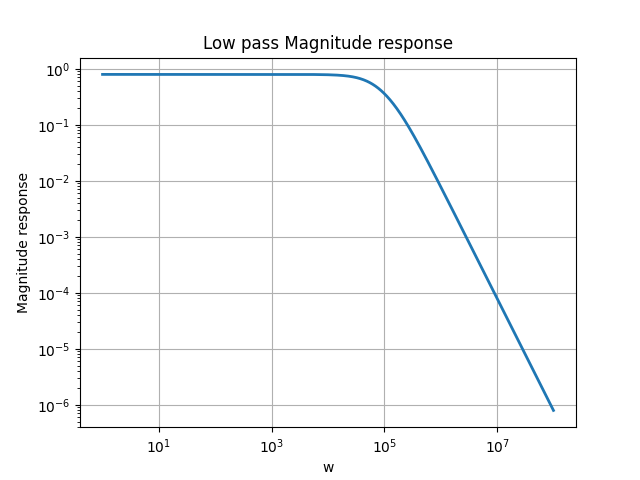
\includegraphics[scale=0.5]{assgn8_plot1.png} 
\caption{Magnitude response of lowpass filter}
\label{fig1}
\end{figure}

\subsection*{Question 1}
The unit step response for the lowpass filter:
\lstinputlisting[language=Python,firstline=82,lastline=86]{week8_soln.py}

\begin{figure}[!tbh]
\centering
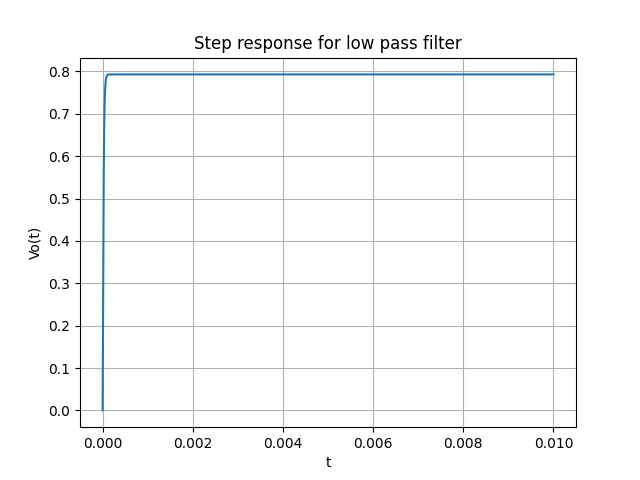
\includegraphics[scale=0.5]{assgn8_plot2.png} 
\caption{Unit step response of lowpass filter}
\label{fig2}
\end{figure}

\subsection*{Question 2}
We give a sum of two sinusoids of different sinusoids as the input to the lowpass filter.
\begin{equation*}
 V_i(t)=[sin(2000 \pi t) + cos(2×10^6 \pi t)]u_o(t)
\end{equation*}
 
\lstinputlisting[language=Python,firstline=46,lastline=52]{week8_soln.py}

\begin{figure}[!tbh]
\centering
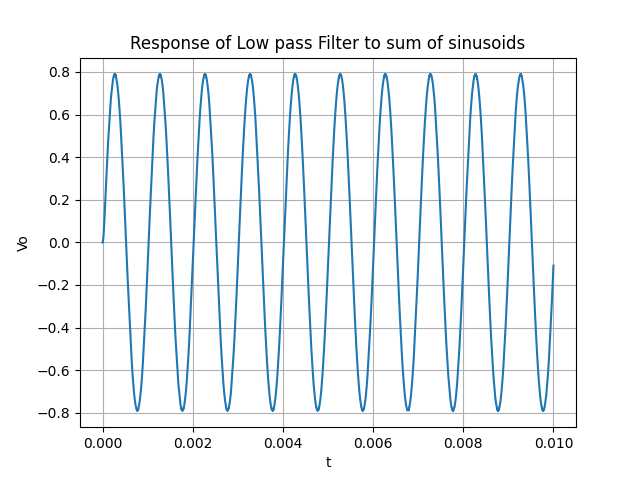
\includegraphics[scale=0.5]{assgn8_plot3.png} 
\caption{Response of lowpass filter to the sum of sinusoids}
\label{fig3}
\end{figure}

\section*{Analysis of highpass filters}
The given circuit specified is a highpass filter.After doing the modified nodal analysis and simplifying the equations , we get:
\newline
$\begin{bmatrix}
    0   & -1 & 0  & -1/G \\
    \frac{sC_2R_3}{sC_2R_3+1}  & 0 & -1 & 0\\
    0  & G & -G & 1 \\
    -sC_2-\frac{1}{R1} - sC_1 & 0 & sC_2 & \frac{1}{R1}
\end{bmatrix}$
$\begin{bmatrix}
    V_1\\
    V_p\\
    V_m \\
    V_o
\end{bmatrix}$
=
$\begin{bmatrix}
    0 \\
    0 \\
    0 \\
    \frac{-V_i(s)}{R_1} \\
    
\end{bmatrix}$

\subsection*{Question 2.2}
We plot the response of the highpass filter to the sum of the two sinusoids.
\begin{figure}[!tbh]
\centering
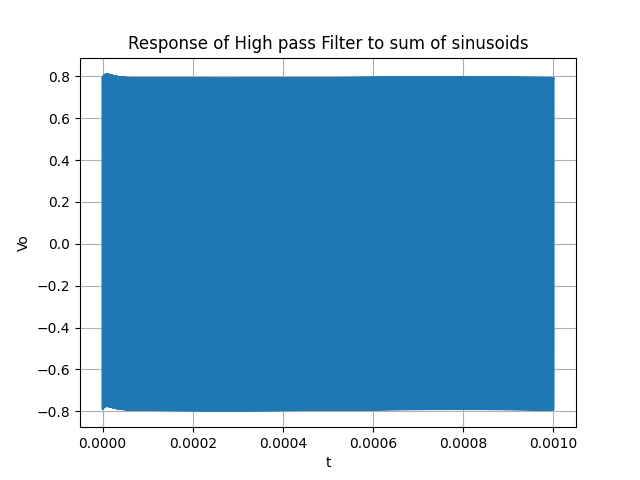
\includegraphics[scale=0.5]{assgn8_plot5.png} 
\caption{Response of highpass filter to the sum of sinusoids}
\label{fig4}
\end{figure}

\subsection*{Question 3}
The magnitude bode plot of the highpass filter looks like:
\begin{figure}[!tbh]
\centering
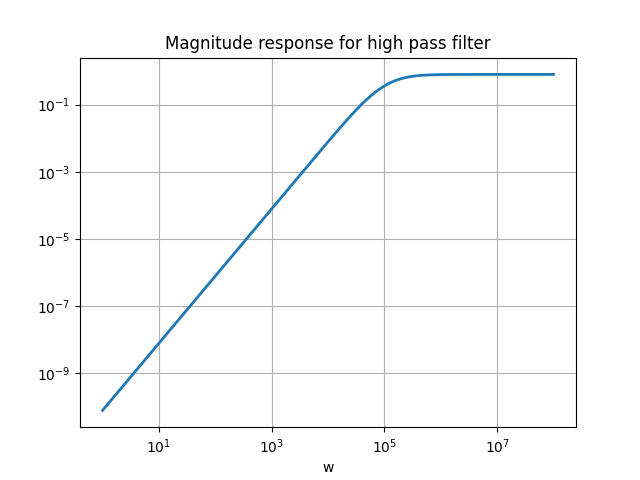
\includegraphics[scale=0.5]{assgn8_plot4.png} 
\caption{Magnitude response of highpass filter}
\label{fig5}
\end{figure}

\subsection*{Question 4}
The high frequency damped sinusoid used here is:
\begin{equation*}
 V_i(t)=cos(10^7 t).exp(-3*10^3 t).u_o(t)
\end{equation*}
\newline
The low frequency damped sinusoid used here is:
\begin{equation*}
 V_i(t)=cos(10^3 t).exp(-10t).u_o(t)
\end{equation*}

\begin{figure}[!tbh]
\centering
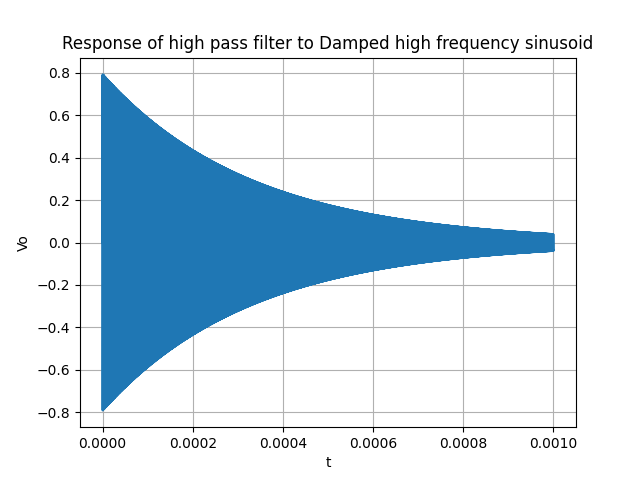
\includegraphics[scale=0.5]{assgn8_plot6.png} 
\caption{Output of high frequency damped sinusoid to highpass filter}
\label{fig6}
\end{figure}

\begin{figure}[!tbh]
\centering
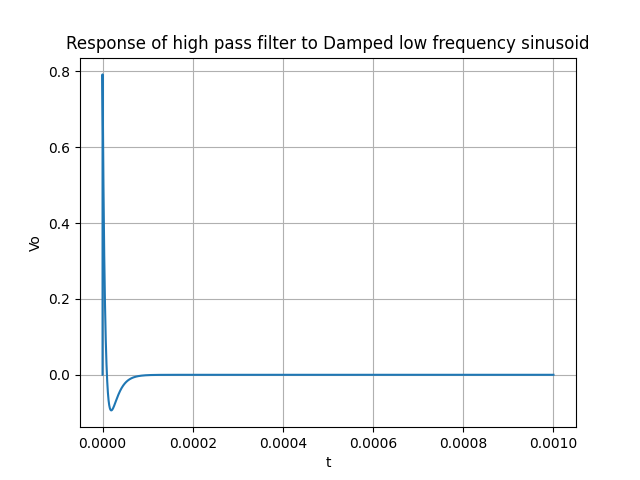
\includegraphics[scale=0.5]{assgn8_plot7.png} 
\caption{Output of low frequency damped sinusoid to highpass filter}
\label{fig7}
\end{figure}

The high pass filter responds by quickly attenuating the input. This is because the input frequency is below the cutoff frequency, so the output goes to 0 very fast.


\subsection*{Question 5}

\begin{figure}[!tbh]
\centering
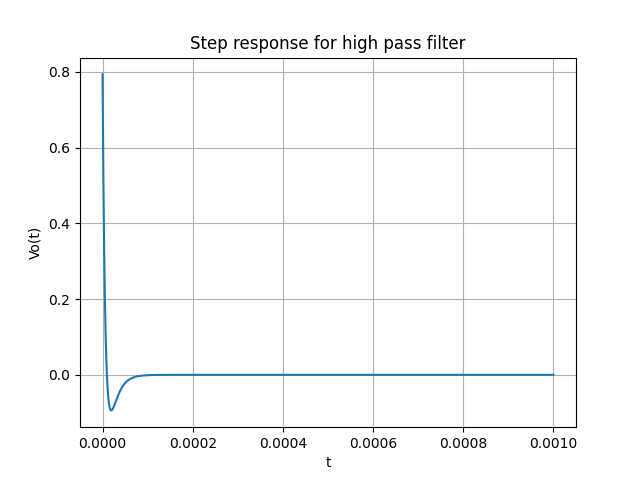
\includegraphics[scale=0.5]{assgn8_plot8.png} 
\caption{Step response of highpass filter}
\label{fig8}
\end{figure}

The unit step response, as expected is high at t=0 when there is an abrupt
change in the input. Since there is no other change at large time values outside
the neighbourhood of 0, the Fourier transform of the unit step has high values
near 0 frequency, which the high pass filter attenuates.

\section*{Conclusion}
In conclusion, the sympy module has allowed us to analyse quite complicated circuits by analytically solving their node equations. We then interpreted the solutions by plotting time domain responses using the signals toolbox. Thus, sympy combined with the scipy.signal module is a very useful toolbox for analyzing complicated systems like the active filters in this assignment.

\end{document}